\chapter{Технологическая часть}

В данном разделе представлены архитектура приложения, средства разработки программного обеспечения, детали реализации и способы взаимодействия с программным продуктом.

\section{Архитектура приложения}

Предполагается, что разрабатываемое приложение является микросервисом одного большего сервиса (LMS). Доступ к данным, хранящимся в приложении будет получен с помощью REST API.

Серверная часть коммуницирует с базами данных при помощи специализированных коннекторов, позволяющих делать запросы к базе данных на языке программирования, который используется для разработки приложения. 

Общая схема архитектура приложения представлена на рисунке \ref{img:app-architecture}.

\begin{figure}[h!]
	\begin{center}
		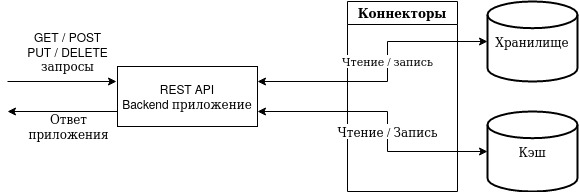
\includegraphics[scale=0.8]{img/app-arch.jpg}
	\end{center}
	\captionsetup{justification=centering}
	\caption{Схема архитектуры приложения}
	\label{img:app-architecture}
\end{figure}

\section{Средства реализации}

Для разработки серверной части был выбран язык программирования Python \cite{python}. Данный выбор обусловлен простотой языка и развертыванием REST-приложений на нём. Также в Python имеется очень тесная интеграция с СУБД PostgreSQL, которая будет использоваться для хранения данных о рабочей программы дисциплины. Язык Python имеет коннекторы для платформы in-memory вычислений Tarantool. Для реализации REST API был выбран фреймворк Flask \cite{flask}.

Для коммуникации серверной части приложения с базами данных были использованы коннекторы: python-tarantool \cite{python-tarantool} для Tarantool и psycopg2 \cite{psycopg2} для PostgreSQL.

Для упаковки приложения в готовый продукт была выбрана система контейнеризации Docker \cite{docker}. С помощью Docker, можно создать изолированную среду для программного обеспечения, которое можно будет развернуть на различных операционных система без дополнительного вмешательства для обеспечения совместимости.

Тестирование программного продукта производилось с помощью фреймворка pytest \cite{pytest}. Данный фреймворк позволяет писать как модульные, так и функциональные тесты. Для тестирования ПО был реализован ряд функциональных тестов.

\section{Детали реализации}

В листингах \ref{lst:app} -- \ref{lst:db-tarantool} представлены листинги взаимодействия клиента с сервером и обработка запросов клиента, взаимодействия приложения с базами данных и кэширования данных.

\begin{lstlisting}[label=lst:app, caption=Листинг взаимодействия клиента с сервером, language=python]
import logging
import time

from flask import Flask, request
import psycopg2

import db.models as m
from db.cache.cache import CacheLRU
from db.utils import Utils

from services.controller import Controller
from services.handler import RequestHandler
from services.document_parser import DocumentParser

app = Flask(__name__)
app.config['JSON_AS_ASCII'] = False

# Waiting for database initialization
time.sleep(1)
cache = CacheLRU()
controller = Controller()


@app.route("/rpd/save", methods=["POST"])
def upload_from_file():
	logging.info(f"/rpd/save router called")
	repo_psql = controller.discipline_work_program_repo_psql
	filename = request.get_json()["filename"]

	try:
		parser = DocumentParser(filename)
		model = parser.get_discipline_program()
		model.id = repo_psql.save(model)
		model = Utils.save_discipline_fields(model, controller.psql_repos)
	except Exception as err:
		logging.error(err)
		return RequestHandler.error_response(500, err)
	
	return RequestHandler.success_response(data=model)


@app.route("/rpd/<id>", methods=["GET"])
def get_dpw_by_id(id=None):
	logging.info(f"/dpw/{id} (GET) router called")
	repos = {
		"storage": controller.psql_repos,
		"cache": controller.tarantool_repos,
	}

	try:
		model = cache.get_by_primary(int(id), "discipline_work_program", repos)
		model = Utils.collect_discipline_fields(model, cache, repos)
	except Exception as err:
		logging.error(err)
		return RequestHandler.error_response(500, err)
	
	return RequestHandler.success_response(data=model)


@app.route("/rpd/<id>", methods=["DELETE"])
def remove_dpw_by_id(id=None):
	logging.info(f"/rpd/{id} (DELETE) router called")
	repo_psql = controller.discipline_work_program_repo_psql
	repo_tarantool = controller.discipline_work_program_repo_tarantool
	repos = {
		"storage": controller.psql_repos,
		"cache": controller.tarantool_repos,
	}
	
	try:
		model = cache.get_by_primary(int(id), "discipline_work_program", repos)
		Utils.remove_discipline_fields(model, cache, repos)
		repo_psql.remove(model.id)
	except Exception as err:
		logging.error(err)
		return RequestHandler.error_response(500, err)
	
	return RequestHandler.success_response(
		message=f"Work program of discipline with id = {id} successfully deleted")


@app.route("/rpd/<id>", methods=["PUT"])
def edit_dpw_by_id(id=None):
	logging.info(f"/rpd/{id} (PUT) router called")
	repo_psql = controller.discipline_work_program_repo_psql
	repo_tararntool = controller.discipline_work_program_repo_tarantool
	
	try:
		model = repo_psql.edit(id=int(id), fields=request.get_json())
	except Exception as err:
		logging.error(err)
		return RequestHandler.error_response(500, err)
	
	return RequestHandler.success_response(
		message=f"Work program of discipline with id = {id} successfully changed")


@app.route("/cache/clear", methods=["PUT"])
def clear_cache():
	logging.info(f"Clear cache router called")
	cache_repos = controller.tarantool_repos
	
	try:
		cache.clear(cache_repos, cache_repos["discipline_work_program"].connection)
	except Exception as err:
		logging.error(err)
		return RequestHandler.error_response(500, err)
	
	return RequestHandler.success_response(message=f"Cache successfully cleared")


@app.route("/cache/size", methods=["GET"])
def cache_size():
	logging.info(f"Get cache size router called")
	cache_repos = controller.tarantool_repos

	try:
		size = cache.get_cache_size(cache_repos["discipline_work_program"].connection)
	except Exception as err:
		logging.error(err)
		return RequestHandler.error_response(500, err)
	
	return RequestHandler.success_response(message=f"Cache size is {size}")


@app.route("/cache/<id>", methods=["DELETE"])
def remove_from_cache(id=None):
logging.info(f"Remove from cache with id = {id} router called")
	space_name = request.get_json()["space_name"]
	
	try:
		cache.remove(int(id), space_name, controller.tarantool_repos[space_name])
	except Exception as err:
		logging.error(err)
		return RequestHandler.error_response(500, err)

	return RequestHandler.success_response(message=f"Cache successfully cleared")


@app.errorhandler(404)
def page_not_found(error):
	return RequestHandler.error_response(404, "Invalid URL!")

if __name__ == "__main__":
	app.run(host='0.0.0.0')
\end{lstlisting}

\begin{lstlisting}[label=lst:cache, caption=Листинг модуля кэширования данных с политикой вытеснения LRU, language=python]
from datetime import datetime
from heapq import heappush as insert_queue, heappop as extract_maximum

from db.utils import Utils

class CacheLRU():
	def __init__(self, max_size=100):
		self.max_size = max_size
		self.current_size = None
		self.time_queue = []
	
	def get_by_primary(self, key, space_name, repos):
		current_time = datetime.timestamp(datetime.now())
		cache_repo = repos["cache"][space_name]
		storage_repo = repos["storage"][space_name]
		
		if self.current_size is None:
			self.current_size = self.get_cache_size(cache_repo.connection)
		
		cached_object = cache_repo.get_by_id(key)
		if cached_object is not None:
			insert_queue(self.time_queue, (current_time, key, space_name))
			return cached_object
		
		if self.current_size >= self.max_size:
			min_key, cached_space_name = extract_maximum(self.time_queue)[1:]
			cache_repo.remove(min_key)
			self.decrement_cache_size(cache_repo.connection)
		
		obj = storage_repo.get_by_id(key)
		cache_repo.save(obj)
		self.increment_cache_size(cache_repo.connection)
		insert_queue(self.time_queue, (current_time, key, space_name))
		
		return obj
	
	def get_by_filter(self, space_name, key, index, repos):
		current_time = datetime.timestamp(datetime.now())
		cache_repo = repos["cache"][space_name]
		storage_repo = repos["storage"][space_name]
		
		if self.current_size is None:
			self.current_size = self.get_cache_size(cache_repo.connection)
		
		cached_objects, primary_keys = cache_repo.get_by_filter(index, key)
		if cached_objects is not None:
			for obj, primary_key in zip(cached_objects, primary_keys):
				insert_queue(self.time_queue, (current_time, primary_key, space_name))
		
		total_cnt = storage_repo.get_objects_count_by_filter(index, key)
		objects_left = total_cnt if cached_objects is None else total_cnt - len(cached_objects)
		if objects_left == 0:
			return cached_objects
		
		if objects_left == total_cnt:
			primary_keys = [-1] # Full-scan confirmed
	
		while self.current_size + objects_left >= self.max_size:
			min_key, space_name = extract_maximum(self.time_queue)[1:]
			repos["cache"][space_name].remove(min_key)
			self.decrement_cache_size(cache_repo.connection)
		
		filter_str = Utils.get_noncached_filter_string(len(primary_keys), index)
		objects, primary_keys = storage_repo.get_by_filter(filter_str, tuple(map(int, [key] + primary_keys)))
		
		for obj, primary_key in zip(objects, primary_keys):
			cache_repo.save(obj)
			self.increment_cache_size(cache_repo.connection)
			insert_queue(self.time_queue, (datetime.timestamp(datetime.now()), primary_key, space_name))
		
		return objects
	
	def insert(self, key, obj, repo):
		current_time = datetime.timestamp(datetime.now())
	
		if self.current_size is None:
			self.current_size = self.get_cache_size(repo.connection)
	
		if self.current_size >= self.max_size:
			key = extract_maximum(self.time_queue)[-1]
			repo.remove(key)
	
		insert_queue(self.time_queue, (current_time, key, repo._meta["space_name"]))
		self.increment_cache_size(repo.connection)
		repo.save(obj)
	
	def remove(self, key, space_name, repo):
		if self.current_size is None:
			self.current_size = self.get_cache_size(repo.connection)
	
		if repo.remove(key) is not None:
			self.time_queue = list(filter(lambda x: x[1] != key or x[2] != space_name, self.time_queue))
			self.decrement_cache_size(repo.connection)
	
	def update(self, key, repo):
		obj = self.remove(key, repo)
		self.insert(key, obj, repo)
	
	def clear(self, repos, connection):
		for key in repos:
			space_name = repos[key]._meta["space_name"]
			connection.call(f"box.space.{space_name}:truncate", ())
	
		self.current_size = 0
		connection.space("cache_size").replace((1, 0))
	
	def increment_cache_size(self, connection):
		self.current_size += 1
		connection.space("cache_size").replace((1, self.current_size))
	
	def decrement_cache_size(self, connection):
		self.current_size -= 1
		connection.space("cache_size").replace((1, self.current_size))
	
	def get_cache_size(self, connection):
		return connection.space("cache_size").select()[0][1]
\end{lstlisting}

\begin{lstlisting}[label=lst:db-postgresql, caption=Листинг модуля взаимодействия c СУБД PostgreSQL, language=python]
import logging
import psycopg2

from db.utils import Utils
from db.repos.abstract import AbstractRepo
import db.models as models

class DisciplineWorkProgramRepoPSQL(AbstractRepo):
	def __init__(self, connection):
		self.connection = connection
		self._meta = {
		"table_name": "discipline_work_program",
		"field_names": {"id": int, "name": str, "author": str, "competency": str}
		}
	
	def save(self, model):
		if not isinstance(model, models.DisciplineWorkProgram):
			logging.error("Trying to save DisciplineWorkProgram object of invalid type")
			raise TypeError("Expected object is instance of DisciplineWorkProgram")
	
		with self.connection.cursor() as cursor:
			insert_names = Utils.get_insert_fields(self._meta["field_names"])
			cursor.execute(
				f"INSERT INTO {self._meta['table_name']} {insert_names} VALUES (%s, %s, %s) RETURNING id",
				(model.name, model.author, model.competency),
			)
	
			self.connection.commit()
		return cursor.fetchone()[0] # Return id of new row in database
	
	def get_by_id(self, model_id):
		with self.connection.cursor() as cursor:
			cursor.execute(f"SELECT * FROM {self._meta['table_name']} WHERE id = %s", (model_id,))
			orm_objects = cursor.fetchall()
	
			if len(orm_objects) == 0:
				raise ValueError(f"Work program of discipline with id = {model_id} doesn't exists")
	
		return models.DisciplineWorkProgram(*orm_objects[0])
	
	def get_by_filter(self, filter, keys):
		with self.connection.cursor() as cursor:
		cursor.execute(f"SELECT * FROM {self._meta['table_name']} WHERE {filter}", keys)
	
		orm_objects = cursor.fetchall()
		if len(orm_objects) == 0:
			return None, None
	
		models_list = list()
		primary_keys = list()
		for obj in orm_objects:
			model = models.DisciplineWorkProgram(*obj)
			models_list.append(model)
			primary_keys.append(model.id)
	
		return models_list, primary_keys
	
	def get_objects_count_by_filter(self, field, key):
		with self.connection.cursor() as cursor:
			cursor.execute(f"SELECT COUNT(*) FROM {self._meta['table_name']} WHERE {field} = %s", (key,))
			orm_objects = cursor.fetchall()
	
		if len(orm_objects) == 0:
			return None
	
		return orm_objects[0][0]
	
	def get_all(self):
		with self.connection.cursor() as cursor:
			cursor.execute(f"SELECT * FROM {self._meta['table_name']}")
			orm_objects = cursor.fetchall()
	
		models_list = list()
		for obj in orm_objects:
			models_list.append(models.DisciplineWorkProgram(*obj))
	
		return models_list
		
	def remove(self, id):
		with self.connection.cursor() as cursor:
			cursor.execute(f"DELETE FROM {self._meta['table_name']} WHERE id = %s", (id,))
			if cursor.rowcount == 0:
				raise ValueError(f"Work program of discipline with id = {id} doesn't exists.")
	
			self.connection.commit()
	
	def edit(self, *args, **kwargs):
		obj_id = kwargs['id']
		updated_args_str, updated_args = Utils.get_psql_update_args(kwargs['fields'])
	
		with self.connection.cursor() as cursor:
			cursor.execute(
				f"UPDATE {self._meta['table_name']} SET {updated_args_str} WHERE id = %s",
				(updated_args, *obj_id,)
			)
	
		self.connection.commit()


class LearningOutcomesRepoPSQL(AbstractRepo):
	def __init__(self, connection):
		self.connection = connection
		self._meta = {
			"table_name": "learning_outcomes",
			"field_names": {
				"id": int,
				"discipline_id": int,
				"competency_code": str,
				"formulation": str,
				"results": str,
				"forms_and_methods": str,
			}
		}
	
	def save(self, model):
		if not isinstance(model, models.LearningOutcomes):
			logging.error("Trying to save LearningOutcomes object of invalid type")
			raise TypeError("Expected object is instance of LearningOutcomes")
		
		with self.connection.cursor() as cursor:
			insert_names = Utils.get_insert_fields(self._meta["field_names"])
			cursor.execute(
				f"INSERT INTO {self._meta['table_name']} {insert_names} VALUES (%s, %s, %s, %s, %s) RETURNING id", (
				model.discipline_id, model.competency_code,
				model.formulation, model.results, model.forms_and_methods
			),
		)
		
			self.connection.commit()
		return cursor.fetchone()[0]
	
	def get_by_id(self, model_id):
		with self.connection.cursor() as cursor:
			cursor.execute(f"SELECT * FROM {self._meta['table_name']} WHERE id = %s", (model_id,))
			orm_objects = cursor.fetchall()
		
			if len(orm_objects) == 0:
				raise ValueError(f"Learning outcomes of discipline with id = {model_id} doesn't exists")
		
		return models.LearningOutcomes(*orm_objects[0])
		
	def get_by_filter(self, filter, keys):
		with self.connection.cursor() as cursor:
			cursor.execute(f"SELECT * FROM {self._meta['table_name']} WHERE {filter}", keys)
	
			orm_objects = cursor.fetchall()
			if len(orm_objects) == 0:
				return None, None
		
		models_list = list()
		primary_keys = list()
		for obj in orm_objects:
			model = models.LearningOutcomes(*obj)
			models_list.append(model)
			primary_keys.append(model.id)
			
		return models_list, primary_keys
	
	def get_objects_count_by_filter(self, field, key):
		with self.connection.cursor() as cursor:
			cursor.execute(f"SELECT COUNT(*) FROM {self._meta['table_name']} WHERE {field} = %s", (key,))
			orm_objects = cursor.fetchall()
		
		if len(orm_objects) == 0:
			return None
		
		return orm_objects[0][0]
	
	def get_all(self):
		with self.connection.cursor() as cursor:
			cursor.execute(f"SELECT * FROM {self._meta['table_name']}")
			orm_objects = cursor.fetchall()
		
		models_list = list()
		for obj in orm_objects:
			models_list.append(models.LearningOutcomes(*obj))
		
		return models_list
	
	def remove(self, id):
		with self.connection.cursor() as cursor:
			cursor.execute(f"DELETE FROM {self._meta['table_name']} WHERE id = %s", (id,))
			if cursor.rowcount == 0:
				raise ValueError(f"Learning outcomes of discipline with id = {id} doesn't exists.")
			
			self.connection.commit()
	
	def edit(self, *args, **kwargs):
		obj_id = kwargs['id']
		updated_args_str, updated_args = Utils.get_psql_update_args(kwargs['fields'])
		
		with self.connection.cursor() as cursor:
			cursor.execute(
				f"UPDATE {self._meta['table_name']} SET {updated_args_str} WHERE id = %s",
				(updated_args, *obj_id,)
			)
		
		self.connection.commit()


class EducationalProgramRepoPSQL(AbstractRepo):
	def __init__(self, connection):
		self.connection = connection
		self._meta = {
			"table_name": "educational_program",
			"interconnection_table_name": "discipline_educational_program",
			"ict_field_name": "educational_program_id",
			"field_names": {
			"id": int,
			"name": str
			}
		}
	
	def save(self, model):
		if not isinstance(model, models.EducationalProgram):
			logging.error("Trying to save EducationalProgram object of invalid type")
			raise TypeError("Expected object is instance of EducationalProgram")
	
		with self.connection.cursor() as cursor:
			try:
				cursor.execute(
					f"INSERT INTO {self._meta['table_name']} VALUES (%s, %s) RETURNING id",
					(model.id, model.name))
			except psycopg2.errors.UniqueViolation:
				self.connection.commit()
				model.id = self.get_by_id(model.id).id
			
			cursor.execute(f"INSERT INTO {self._meta['interconnection_table_name']} \
			VALUES (%s, %s)", (model.discipline_id, model.id))
			
			self.connection.commit()
			
		return model.id
	
	def get_by_id(self, model_id):
		with self.connection.cursor() as cursor:
			cursor.execute(f"SELECT * FROM {self._meta['table_name']} WHERE id = %s", (model_id,))
			orm_objects = cursor.fetchall()
		
		if len(orm_objects) == 0:
			raise ValueError(f"Educational program with id = {model_id} doesn't exists")
		
		return models.EducationalProgram(*orm_objects[0])
	
	def get_by_filter(self, filter, keys):
		with self.connection.cursor() as cursor:
			cursor.execute(f"\
				SELECT id, name FROM {self._meta['interconnection_table_name']} \
				JOIN {self._meta['table_name']} ON (id = {self._meta['ict_field_name']}) \
				WHERE {filter}", keys)
		
			orm_objects = cursor.fetchall()
			if len(orm_objects) == 0:
				return None, None
		
		models_list = list()
		primary_keys = list()
		for obj in orm_objects:
			model = models.EducationalProgram(*obj)
			model.discipline_id = keys[0]
			models_list.append(model)
			primary_keys.append(model.id)
		
		return models_list, primary_keys
	
	def get_objects_count_by_filter(self, field, key):
		with self.connection.cursor() as cursor:
			cursor.execute(f"SELECT COUNT(*) FROM {self._meta['table_name']} WHERE {field} = %s", (key,))
			orm_objects = cursor.fetchall()
		
		if len(orm_objects) == 0:
			return None
		
		return orm_objects[0][0]
	
	def get_all(self):
		with self.connection.cursor() as cursor:
			cursor.execute(f"SELECT * FROM {self._meta['table_name']}")
			orm_objects = cursor.fetchall()
		
		models_list = list()
		for obj in orm_objects:
			models_list.append(models.EducationalProgram(*obj))
		
		return models_list
	
	def remove(self, id, *args, **kwargs):
		with self.connection.cursor() as cursor:
			cursor.execute(
				f"DELETE FROM {self._meta['interconnection_table_name']} WHERE discipline_id = %s",
				(kwargs['discipline_id'],))
		
			cursor.execute(f"DELETE FROM {self._meta['table_name']} WHERE id = %s", (id,))
			if cursor.rowcount == 0:
				raise ValueError(f"Educational program of discipline with id = {id} doesn't exists.")
		
		self.connection.commit()
	
	def edit(self, *args, **kwargs):
		obj_id = kwargs['id']
		updated_args_str, updated_args = Utils.get_psql_update_args(kwargs['fields'])
		
		with self.connection.cursor() as cursor:
			cursor.execute(
				f"UPDATE {self._meta['table_name']} SET {updated_args_str} WHERE id = %s",
				(updated_args, *obj_id,)
			)
		
		self.connection.commit()


class DisciplineScopeRepoPSQL(AbstractRepo):
	def __init__(self, connection):
		self.connection = connection
		self._meta = {
			"table_name": "discipline_scope_semester",
			"field_names": {
				"id": int,
				"discipline_id": int,
				"semester_number": int,
				"credit_units": int,
				"total_hours": int,
				"lectures_hours": int,
				"seminars_hours": int,
				"laboratory_work_hours": int,
				"independent_work_hours": int,
				"certification_type": str
			}
		}
	
	def save(self, model):
		if not isinstance(model, models.DisciplineScope):
			logging.error("Trying to save DisciplineScope object of invalid type")
			raise TypeError("Expected object is instance of DisciplineScope")
		
		with self.connection.cursor() as cursor:
			insert_names = Utils.get_insert_fields(self._meta["field_names"])
			cursor.execute(
				f"INSERT INTO {self._meta['table_name']} {insert_names} VALUES \
					(%s, %s, %s, %s, %s, %s, %s, %s, %s) RETURNING id", (
					model.discipline_id, model.semester_number, model.credit_units,
					model.total_hours, model.lectures_hours, model.seminars_hours,
					model.laboratory_hours, model.independent_hours, model.certification_type
				),
			)
		
			self.connection.commit()
		return cursor.fetchone()[0]
	
	def get_by_id(self, model_id):
		with self.connection.cursor() as cursor:
			cursor.execute(f"SELECT * FROM {self._meta['table_name']} WHERE id = %s", (model_id,))
			orm_objects = cursor.fetchall()
		
		if len(orm_objects) == 0:
			raise ValueError(f"Scope of discipline with id = {model_id} doesn't exists")
		
		return models.DisciplineScope(*orm_objects[0])
		
	def get_by_filter(self, filter, keys):
		with self.connection.cursor() as cursor:
			cursor.execute(f"SELECT * FROM {self._meta['table_name']} WHERE {filter}", keys)
		
			orm_objects = cursor.fetchall()
			if len(orm_objects) == 0:
				return None, None
		
		models_list = list()
		primary_keys = list()
		for obj in orm_objects:
			model = models.DisciplineScope(*obj)
			models_list.append(model)
			primary_keys.append(model.id)
		
		return models_list, primary_keys
	
	def get_objects_count_by_filter(self, field, key):
		with self.connection.cursor() as cursor:
			cursor.execute(f"SELECT COUNT(*) FROM {self._meta['table_name']} WHERE {field} = %s", (key,))
			orm_objects = cursor.fetchall()
		
		if len(orm_objects) == 0:
			return None
		
		return orm_objects[0][0]
	
	def get_all(self):
		with self.connection.cursor() as cursor:
			cursor.execute(f"SELECT * FROM {self._meta['table_name']}")
			orm_objects = cursor.fetchall()
		
		models_list = list()
		for obj in orm_objects:
			models_list.append(models.DisciplineScope(*obj))
		
		return models_list
	
	def remove(self, id):
		with self.connection.cursor() as cursor:
			cursor.execute(f"DELETE FROM {self._meta['table_name']} WHERE id = %s", (id,))
			if cursor.rowcount == 0:
				raise ValueError(f"Scope of discipline with id = {id} doesn't exists.")
		
		self.connection.commit()
		
	def edit(self, *args, **kwargs):
		obj_id = kwargs['id']
		updated_args_str, updated_args = Utils.get_psql_update_args(kwargs['fields'])
		
		with self.connection.cursor() as cursor:
			cursor.execute(
				f"UPDATE {self._meta['table_name']} SET {updated_args_str} WHERE id = %s",
				(updated_args, *obj_id,)
			)
		
		self.connection.commit()


class DisciplineModuleRepoPSQL(AbstractRepo):
	def __init__(self, connection):
		self.connection = connection
		self._meta = {
			"table_name": "discipline_module",
			"field_names": {
				"id": int,
				"discipline_id": int,
				"name": str,
				"semester_number": int,
				"lectures_hours": int,
				"seminars_hours": int,
				"laboratory_work_hours": int,
				"independent_work_hours": int,
				"min_scores": int,
				"max_scores": int,
				"competency_codes": str
			}
		}
	
	def save(self, model):
		if not isinstance(model, models.DisciplineModule):
			logging.error("Trying to save DisciplineModule object of invalid type")
			raise TypeError("Expected object is instance of DisciplineModule")
		
		with self.connection.cursor() as cursor:
			insert_names = Utils.get_insert_fields(self._meta["field_names"])
			cursor.execute(
				f"INSERT INTO {self._meta['table_name']} {insert_names} VALUES \
					(%s, %s, %s, %s, %s, %s, %s, %s, %s, %s) RETURNING id", (
					model.discipline_id, model.name, model.semester_number,
					model.lectures_hours, model.seminars_hours,
					model.laboratory_hours, model.independent_hours, model.min_score,
					model.max_score, model.competency_code
					),
				)
		
			self.connection.commit()
			return cursor.fetchone()[0]
	
	def get_by_id(self, model_id):
		with self.connection.cursor() as cursor:
			cursor.execute(f"SELECT * FROM {self._meta['table_name']} WHERE id = %s", (model_id,))
			orm_objects = cursor.fetchall()
		
		if len(orm_objects) == 0:
			raise ValueError(f"Module of discipline with id = {model_id} doesn't exists")
		
		return models.DisciplineModule(*orm_objects[0])
	
	def get_by_filter(self, filter, keys):
		with self.connection.cursor() as cursor:
			cursor.execute(f"SELECT * FROM {self._meta['table_name']} WHERE {filter}", keys)
		
			orm_objects = cursor.fetchall()
			if len(orm_objects) == 0:
				return None, None
		
		models_list = list()
		primary_keys = list()
		for obj in orm_objects:
			model = models.DisciplineModule(*obj)
			models_list.append(model)
			primary_keys.append(model.id)
		
		return models_list, primary_keys
	
	def get_objects_count_by_filter(self, field, key):
		with self.connection.cursor() as cursor:
			cursor.execute(f"SELECT COUNT(*) FROM {self._meta['table_name']} WHERE {field} = %s", (key,))
			orm_objects = cursor.fetchall()
		
		if len(orm_objects) == 0:
			return None
		
		return orm_objects[0][0]
	
	def get_all(self):
		with self.connection.cursor() as cursor:
			cursor.execute(f"SELECT * FROM {self._meta['table_name']}")
			orm_objects = cursor.fetchall()
		
		if len(orm_objects) == 0:
			return None
		
		models_list = list()
		for obj in orm_objects:
			models_list.append(models.DisciplineModule(*obj))
		
		return models_list
	
	def remove(self, id):
		with self.connection.cursor() as cursor:
			cursor.execute(f"DELETE FROM {self._meta['table_name']} WHERE id = %s", (id,))
			if cursor.rowcount == 0:
				raise ValueError(f"Module of discipline with id = {id} doesn't exists.")
		
		self.connection.commit()
	
	def edit(self, *args, **kwargs):
		obj_id = kwargs['id']
		updated_args_str, updated_args = Utils.get_psql_update_args(kwargs['fields'])
		
		with self.connection.cursor() as cursor:
			cursor.execute(
				f"UPDATE {self._meta['table_name']} SET {updated_args_str} WHERE id = %s",
				(updated_args, *obj_id,)
			)
		
		self.connection.commit()


class DisciplineMaterialRepoPSQL(AbstractRepo):
	def __init__(self, connection):
		self.connection = connection
		self._meta = {
			"table_name": "discipline_material",
			"field_names": {"id": int, "discipline_id": int, "material": str}
		}
	
	def save(self, model):
		if not isinstance(model, models.DisciplineMaterial):
			logging.error("Trying to save DisciplineMaterial object of invalid type")
			raise TypeError("Expected object is instance of DisciplineMaterial")
		
		with self.connection.cursor() as cursor:
			insert_names = Utils.get_insert_fields(self._meta["field_names"])
			cursor.execute(
				f"INSERT INTO {self._meta['table_name']} {insert_names} VALUES (%s, %s) RETURNING id", (
					model.discipline_id, model.material
				),
			)
		
		self.connection.commit()
		return cursor.fetchone()[0]
	
	def get_by_id(self, model_id):
		with self.connection.cursor() as cursor:
			cursor.execute(f"SELECT * FROM {self._meta['table_name']} WHERE id = %s", (model_id,))
			orm_objects = cursor.fetchall()
		
		if len(orm_objects) == 0:
			raise ValueError(f"Material's of discipline with id = {model_id} doesn't exists")
		
		return models.DisciplineMaterial(*orm_objects[0])
	
	def get_by_filter(self, filter, keys):
		with self.connection.cursor() as cursor:
			cursor.execute(f"SELECT * FROM {self._meta['table_name']} WHERE {filter}", keys)
		
			orm_objects = cursor.fetchall()
			if len(orm_objects) == 0:
				return None, None
		
		models_list = list()
		primary_keys = list()
		for obj in orm_objects:
			model = models.DisciplineMaterial(*obj)
			models_list.append(model)
			primary_keys.append(model.id)
			
		return models_list, primary_keys
	
	def get_objects_count_by_filter(self, field, key):
		with self.connection.cursor() as cursor:
			cursor.execute(f"SELECT COUNT(*) FROM {self._meta['table_name']} WHERE {field} = %s", (key,))
			orm_objects = cursor.fetchall()
	
		if len(orm_objects) == 0:
			return None
	
		return orm_objects[0][0]
	
	def get_all(self):
		with self.connection.cursor() as cursor:
			cursor.execute(f"SELECT * FROM {self._meta['table_name']}")
			orm_objects = cursor.fetchall()
			
			if len(orm_objects) == 0:
				return None
		
		models_list = list()
		for obj in orm_objects:
			models_list.append(models.DisciplineMaterial(*obj))
		
		return models_list
	
	def remove(self, id):
		with self.connection.cursor() as cursor:
			cursor.execute(f"DELETE FROM {self._meta['table_name']} WHERE id = %s", (id,))
			if cursor.rowcount == 0:
				raise ValueError(f"Materials of discipline with id = {id} doesn't exists.")
	
			self.connection.commit()
	
	def edit(self, *args, **kwargs):
		obj_id = kwargs['id']
		updated_args_str, updated_args = Utils.get_psql_update_args(kwargs['fields'])
		
		with self.connection.cursor() as cursor:
			cursor.execute(
				f"UPDATE {self._meta['table_name']} SET {updated_args_str} WHERE id = %s",
				(updated_args, *obj_id,)
			)
		
		self.connection.commit()
\end{lstlisting}

\begin{lstlisting}[label=lst:db-tarantool, caption=Листинг модуля взаимодействия с СУБД Tarantool, language=python]
import logging
from db.utils import Utils
from db.repos.abstract import AbstractRepo
import db.models as models

class DisciplineWorkProgramRepoTarantool(AbstractRepo):
	def __init__(self, connection):
		self.connection = connection
		self._meta = {
			"space_name": "discipline_work_program",
			"field_names": {"id": 1, "name": 2, "author": 3, "competency": 4}
		}
		
		self.space = connection.space(self._meta['space_name'])
	
	def save(self, model):
		if not isinstance(model, models.DisciplineWorkProgram):
			logging.error("Trying to save DisciplineWorkProgram object of invalid type")
			raise TypeError("Expected object is instance of DisciplineWorkProgram")
		
		self.space.insert((model.id, model.name, model.author, model.competency))
	
	def get_by_id(self, model_id):
		obj = self.space.select(model_id)
		if len(obj) == 0:
			return None
		
		return models.DisciplineWorkProgram(*obj[0])
	
	def get_by_filter(self, index, key):
		raw_objects = self.space.select(key, index=index)
		if len(obj) == 0:
			return None, None
		
		models_list = list()
		primary_keys = list()
		for obj in raw_objects:
			model = models.DisciplineWorkProgram(*obj)
			models_list.append(model)
			primary_keys.append(model.id)
		
		return models_list, primary_keys
	
	
	def get_all(self):
		raw_objects = self.space.select()
		if len(raw_objects) == 0:
			return None
		
		models_list = list()
		for obj in raw_objects:
			models_list.append(models.DisciplineWorkProgram(*obj))
		
		return models_list
	
	def remove(self, id):
		obj = self.space.delete(id)
		if len(obj) == 0:
			return None
		
		return obj
	
	def edit(self, *args, **kwargs):
		obj_id = kwargs['id']
		updated_args = Utils.get_tarantool_update_args(kwargs['fields'], self._meta['field_names'])
		
		return self.space.update(obj_id, updated_args)[0]


class LearningOutcomesRepoTarantool(AbstractRepo):
	def __init__(self, connection):
		self.connection = connection
		self._meta = {
			"space_name": "learning_outcomes",
			"field_names": {
				"id": 1,
				"discipline_id": 2,
				"competency_code": 3,
				"formulation": 4,
				"results": 5,
				"forms_and_methods": 6,
			}
		}
		
		self.space = connection.space(self._meta['space_name'])
	
	def save(self, model):
		if not isinstance(model, models.LearningOutcomes):
			logging.error("Trying to save LeraningOutcomes object of invalid type")
			raise TypeError("Expected object is instance of LearningOutcomes")
		
		self.space.insert(tuple(model.__dict__.values()))
	
	def get_by_filter(self, index, key):
		raw_objects = self.space.select(key, index=index)
		if len(raw_objects) == 0:
			return None, None
		
		models_list = list()
		primary_keys = list()
		for obj in raw_objects:
			model = models.LearningOutcomes(*obj)
			models_list.append(model)
			primary_keys.append(model.id)
		
		return models_list, primary_keys
	
	def remove(self, id):
		obj = self.space.delete(id)
		if len(obj) == 0:
			return None
		
		return obj


class DisciplineScopeRepoTarantool(AbstractRepo):
	def __init__(self, connection):
		self.connection = connection
		self._meta = {
			"space_name": "discipline_scope_semester",
			"field_names": {
				"id": 1,
				"discipline_id": 2,
				"semester_number": 3,
				"credit_units": 4,
				"total_hours": 5,
				"lectures_hours": 6,
				"laboratory_work_hours": 7,
				"independent_work_hours": 8,
				"certification_type": 9
			}
		}

		self.space = connection.space(self._meta['space_name'])

	def save(self, model):
		if not isinstance(model, models.DisciplineScope):
			logging.error("Trying to save DisciplineScope object of invalid type")
			raise TypeError("Expected object is instance of DisciplineScope")
		
		self.space.insert(tuple(model.__dict__.values()))
	
	def get_by_filter(self, index, key):
		raw_objects = self.space.select(key, index=index)
		if len(raw_objects) == 0:
			return None, None
		
		models_list = list()
		primary_keys = list()
		for obj in raw_objects:
			model = models.DisciplineScope(*obj)
			models_list.append(model)
			primary_keys.append(model.id)
		
		return models_list, primary_keys
	
	def remove(self, id):
		obj = self.space.delete(id)
		if len(obj) == 0:
			return None
		
		return obj


class DisciplineModuleRepoTarantool(AbstractRepo):
	def __init__(self, connection):
		self.connection = connection
		self._meta = {
			"space_name": "discipline_module",
			"field_names": {
				"id": 1,
				"discipline_id": 2,
				"name": 3,
				"semester_number": 4,
				"lectures_hours": 5,
				"seminars_hours": 6,
				"laboratory_work_hours": 7,
				"independent_work_hours": 8,
				"min_scores": 9,
				"max_scores": 10,
				"competency_codes": 11
			}
		}
	
		self.space = connection.space(self._meta['space_name'])
	
	def save(self, model):
		if not isinstance(model, models.DisciplineModule):
			logging.error("Trying to save DisciplineModule object of invalid type")
			raise TypeError("Expected object is instance of DisciplineModule")
		
		self.space.insert(tuple(model.__dict__.values()))
		
	def get_by_filter(self, index, key):
		raw_objects = self.space.select(key, index=index)
		if len(raw_objects) == 0:
			return None, None
		
		models_list = list()
		primary_keys = list()
		for obj in raw_objects:
			model = models.DisciplineModule(*obj)
			models_list.append(model)
			primary_keys.append(model.id)
		
		return models_list, primary_keys
	
	def remove(self, id):
		obj = self.space.delete(id)
		if len(obj) == 0:
			return None
		
		return obj
	

class DisciplineMaterialRepoTarantool(AbstractRepo):
	def __init__(self, connection):
		self.connection = connection
		self._meta = {
			"space_name": "discipline_material",
			"field_names": {"id": 1, "discipline_id": 2, "materials": 3}
		}
		
		self.space = connection.space(self._meta['space_name'])
	
	def save(self, model):
		if not isinstance(model, models.DisciplineMaterial):
			logging.error("Trying to save DisciplineMaterial object of invalid type")
			raise TypeError("Expected object is instance of DisciplineMaterial")
		
		self.space.insert(tuple(model.__dict__.values()))
	
	def get_by_filter(self, index, key):
		raw_objects = self.space.select(key, index=index)
		if len(raw_objects) == 0:
			return None, None
		
		models_list = list()
		primary_keys = list()
		for obj in raw_objects:
			model = models.DisciplineMaterial(*obj)
			models_list.append(model)
			primary_keys.append(model.id)
		
		return models_list, primary_keys
	
	def remove(self, id):
		obj = self.space.delete(id)
		if len(obj) == 0:
			return None
		
		return obj
\end{lstlisting}


\section{Взаимодействие с приложением}

На рисунках \ref{img:save-example} -- \ref{img:delete-example} представлены примеры запросов к приложению и его ответы.

\begin{figure}[h!]
	\begin{center}
		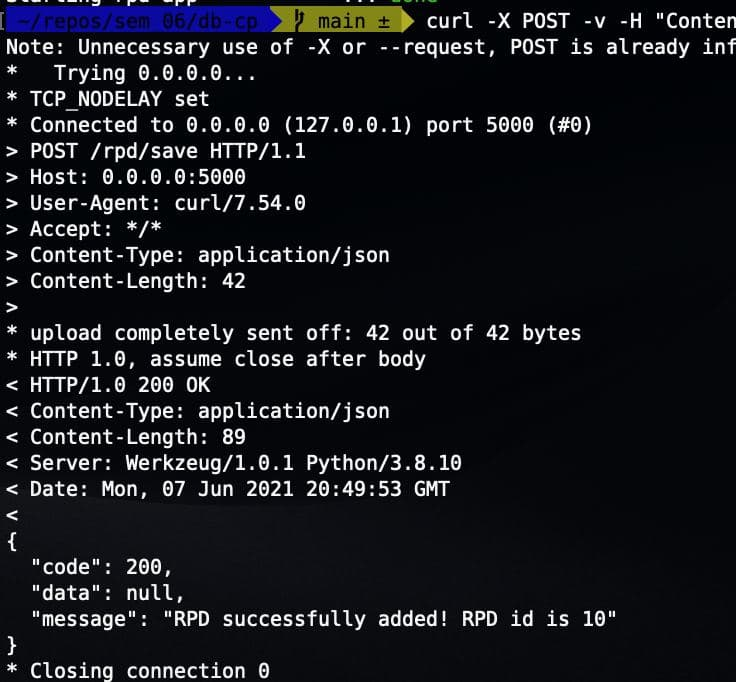
\includegraphics[scale=0.8]{img/save_example.jpg}
	\end{center}
	\captionsetup{justification=centering}
	\caption{Пример сохранения информации о дисциплине посредствам http запроса}
	\label{img:save-example}
\end{figure}

\begin{figure}[h!]
	\begin{center}
		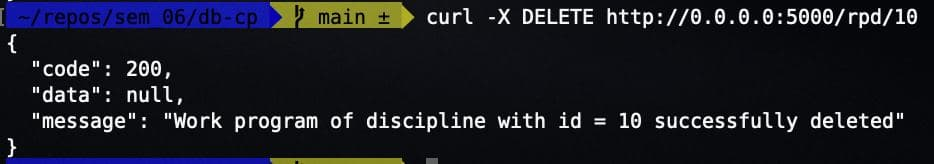
\includegraphics[scale=0.65]{img/delete_example.jpg}
	\end{center}
	\captionsetup{justification=centering}
	\caption{Пример удаления информации о дисциплине посредствам http запроса}
	\label{img:delete-example}
\end{figure}


\begin{figure}[h!]
	\begin{center}
		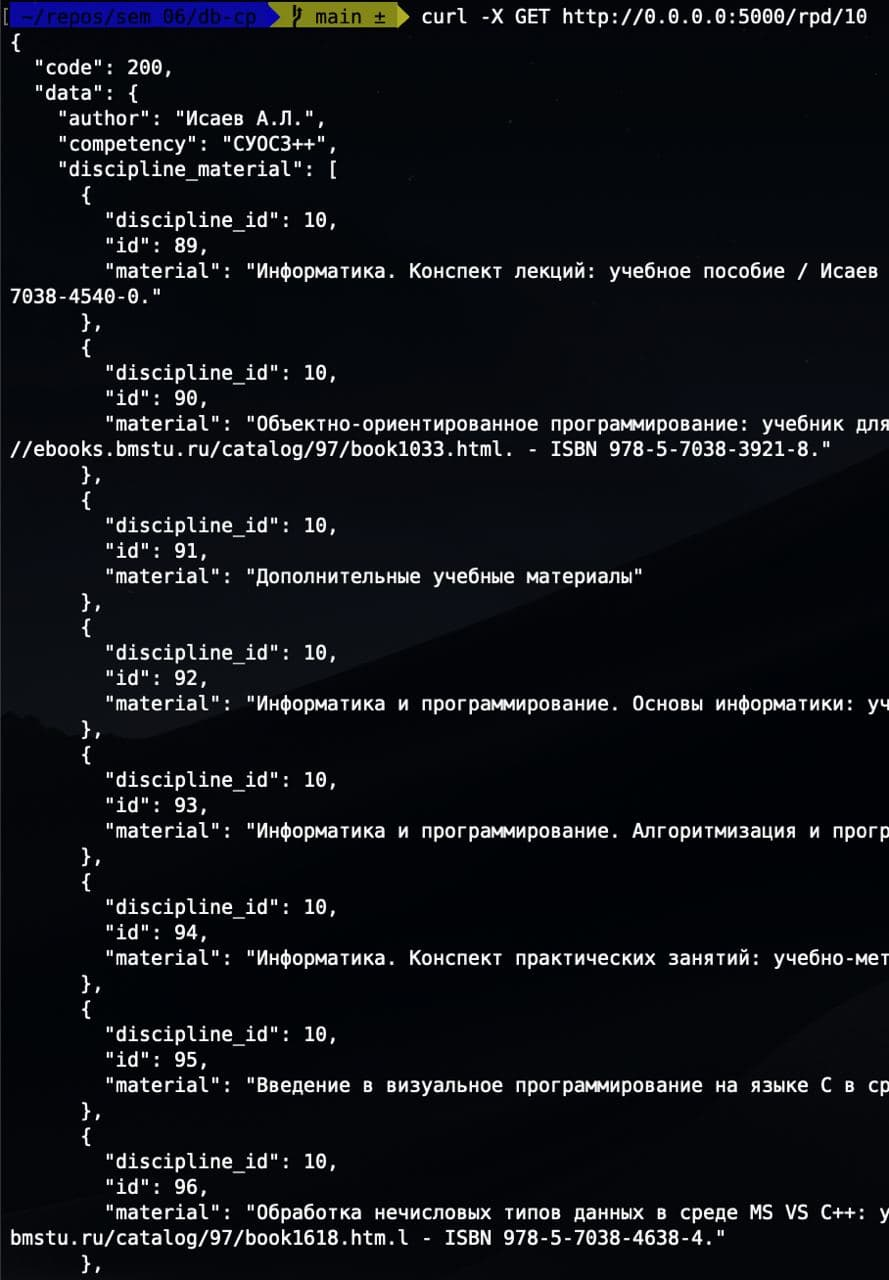
\includegraphics[scale=0.6]{img/get_example.jpg}
	\end{center}
	\captionsetup{justification=centering}
	\caption{Пример получения информации о дисциплине посредствам http запроса}
	\label{img:get-example}
\end{figure}


\section*{Вывод}

В данном разделе были представлена архитектура и средства реализации программного обеспечения, листинги ключевых компонентов системы и пример возвращаемых данных системой.